\documentclass{article}
\usepackage{iclr2026_conference,times}
\input{math_commands.tex}
\usepackage{hyperref}
\usepackage{url}
\usepackage{xcolor}
\usepackage{graphicx}
\usepackage{booktabs}
\usepackage{subcaption}
\usepackage{multirow}
\usepackage{amsmath}
\usepackage{amssymb}

\graphicspath{{../runs/_curve_analysis/}}

\newcommand{\TODO}[1]{{\color{red}\textbf{[TODO: #1]}}}

\title{When Does Autoregressive Pretraining Help Diffusion Language Models?\\
An Interior Optimum at $p_{\mathrm{AR}}{=}0.30$}

\author{Chang-Han Chen \\
University of California, Berkeley\\
Berkeley, CA 94720, USA \\
\texttt{changhanc@berkeley.edu}
}

\iclrfinalcopy
\begin{document}
\maketitle

\begin{abstract}
Diffusion language models (dLMs) are pretraining-expensive but can surpass autoregressive (AR) models when training data is limited. A natural way to amortize the cost is to pretrain autoregressively for a fraction $p_{\mathrm{AR}}$ of the budget, then switch to a (block) diffusion objective for the remainder. Existing A2D conversion recipes implicitly fix $p_{\mathrm{AR}} \approx 0.85\text{--}0.99$: BD3LM uses $p_{\mathrm{MDLM}}{=}0.85$ before block-diffusion finetuning, Dream-7B uses an effective $p_{\mathrm{AR}} \approx 0.97$, and SDAR uses $p_{\mathrm{AR}} \approx 0.999$. We sweep this fraction at 70M-parameter MoE scale on ClimbMix and find a robust \emph{interior optimum} at $p_{\mathrm{AR}}{=}0.30$, invariant in the post-switch BD3 block length for blocks $b \in \{4, 16, 64\}$, and across both AR$\to$BD3 and MDLM$\to$BD3 curricula. The best AR$\to$BD3 run improves over the same-block scratch BD3 baseline by 0.32\% at $b{=}4$ and 1.0\% at $b{=}64$, and beats the BD3LM-style $p_{\mathrm{MDLM}}{=}0.85$ recipe by $\sim$3.3\% at $b{=}4$. We propose a \emph{front-loaded transfer} hypothesis that explains both the interior optimum and its block-length invariance.
\end{abstract}

%=============================================================================
\section{Introduction}
\label{sec:intro}
%=============================================================================

The slogan that ``Diffusion language models are super data learners''~\citep{ni2025diffusionlanguagemodelssuper} is increasingly well-supported: when unique training data is limited, masked-diffusion (MDLM) and block-diffusion (BD3LM) variants of small models eventually surpass AR baselines on downstream evaluations. Unfortunately, dLMs are also pretraining-expensive: per training token, MDLM is roughly $14\times$ less compute-efficient than AR, and uniform-noise diffusion is closer to $32\times$ less efficient. Any-order progressive decoding is simply a strictly harder learning problem than left-to-right next-token prediction.

A natural fix is to spend most of the budget on the cheap AR objective and then \emph{convert} the model to a diffusion objective. This is the standard A2D recipe used in recent works:
\begin{itemize}
\item \textbf{BD3LM}~\citep{arriola2025block} pretrains 850K MDLM steps and finetunes 150K block-diffusion steps at block sizes $\{4, 8, 16\}$, i.e.\ $p_{\mathrm{MDLM}}{=}0.85$, with sequence length $1024$ on OpenWebText.
\item \textbf{Dream-7B}~\citep{dream2025} initializes from Qwen2.5-7B (${\sim}18$T pretraining tokens) and adds $580$B continued-pretraining tokens for diffusion: effective $p_{\mathrm{AR}} \approx 0.969$.
\item \textbf{DiffuLLaMA}~\citep{efficientdlm2025} uses $\sim$65B adaptation tokens on a LLaMA-2 base ($\sim$2T): $p_{\mathrm{AR}} \approx 0.97$.
\item \textbf{SDAR}~\citep{sdar2025} uses only $50$B adaptation tokens on a Qwen3 base ($\sim$36T): $p_{\mathrm{AR}} \approx 0.999$.
\item \textbf{LLaDA-2}~\citep{llada2_2025} performs a 3-phase block-WSD adaptation from a pretrained AR base, again in the very-high-$p_{\mathrm{AR}}$ regime.
\end{itemize}
All five sit at $p_{\mathrm{AR}} \in [0.85, 0.999]$. The implicit hypothesis is ``train autoregressively as long as possible, then briefly adapt to diffusion.'' Two arguments support this on its face: (i)~AR is much cheaper per token, so more AR is more bang-for-buck; (ii)~the smallest BD3 block sizes used at deployment ($b{\in}\{4,8,16\}$) are themselves nearly autoregressive, so a model with strong AR features ought to need only minor adaptation.

This paper challenges that hypothesis. We treat the A2D conversion ratio as a hyperparameter and sweep $p_{\mathrm{AR}}$ over $\{0, 0.30, 0.50, 0.80, 0.90, 0.95\}$, jointly with post-switch block lengths $b \in \{4, 16, 64, 256\}$, at 70M parameters on ClimbMix. We find:

\begin{enumerate}
\item The validation-loss-optimal switch point is \textbf{$p_{\mathrm{AR}}{=}0.30$} for $b \in \{4, 16, 64\}$. Larger $p_{\mathrm{AR}}$ is monotonically worse at every block length except $b{=}256$.
\item This optimum is shared by the MDLM$\to$BD3 curriculum: $p_{\mathrm{MDLM}}{=}0.30$ wins at $b \in \{4, 16, 64\}$, and the BD3LM-published recipe ($p_{\mathrm{MDLM}}{=}0.85$, $b{=}4$) is $\sim$3.3\% behind our $p{=}0.30$ winner at the same model shape and budget.
\item At $b{=}256$ (half of the sequence length), the curriculum framework breaks down entirely: scratch BD3 is competitive or wins, and AR$\to$BD3 with $p_{\mathrm{AR}} > 0$ is monotonically worse. We argue this is the boundary of curriculum transferability.
\end{enumerate}

We propose a \emph{front-loaded transfer + slow target adaptation} hypothesis: AR's marginal value decays concavely after the first ${\sim}30\%$ of training, while BD3 has its own task-specific structure (mask handling, bidirectional intra-block attention) that requires substantial post-switch budget. The interior optimum is where these two marginal values cross, and because the AR phase is identical regardless of post-switch block length, the optimum is approximately invariant in $b$. The exception at $b{=}256$ is predicted because the post-switch task is no longer ``AR-like.''

\textbf{Why this matters.} Existing A2D recipes optimize for inheriting the capabilities of a fixed pretrained AR base, which is a sensible deployment choice but does not minimize the validation loss attainable from a fixed compute budget. Our result is a clean statement about the latter: from-scratch dLM pretraining under a fixed budget should switch \emph{much earlier} than current practice suggests.

%=============================================================================
\section{Related Work}
\label{sec:related}
%=============================================================================

\textbf{Diffusion language models.} MDLM~\citep{sahoo2024simple,shi2024simplified} and BD3LM~\citep{arriola2025block} are the two dLM families we study. BD3LM partitions a sequence into blocks of length $b$, runs left-to-right block decoding, and applies discrete denoising within each block. The block size $b$ interpolates between MDLM ($b = L$, full-sequence diffusion) and AR ($b = 1$).

\textbf{A2D conversion.} Several recent works convert pretrained AR models to diffusion variants at scale: Dream-7B~\citep{dream2025}, DiffuLLaMA / Efficient-DLM~\citep{efficientdlm2025}, SDAR~\citep{sdar2025}, the next-block adaptation framework of~\citet{nbdiff2025}, and LLaDA-2~\citep{llada2_2025}. All start from large off-the-shelf AR models and add a comparatively small diffusion-adaptation phase. We instead study A2D as a from-scratch curriculum, which strictly contains existing A2D as the high-$p_{\mathrm{AR}}$ corner.

\textbf{Super data learners.} \citet{ni2025diffusionlanguagemodelssuper} and \citet{gao2025whatmakes} document that dLMs continue improving past the point where AR overfits in the multi-epoch data-constrained regime. Our curriculum question is orthogonal but motivated by the same setting: if dLMs' advantage is data-constrained, accelerating their per-compute training is the bottleneck.

\textbf{Curriculum and pretraining schedules.} Our front-loaded-transfer interpretation parallels the pretraining-vs-finetuning literature, where features stabilize log-shapedly with budget and additional pretraining shows diminishing returns.

%=============================================================================
\section{Method}
\label{sec:method}
%=============================================================================

\subsection{Curriculum framework}

Let $T$ be the total optimizer-step budget. A curriculum is parameterized by $(p, b)$ where $p \in [0, 1]$ is the source-objective fraction and $b$ is the post-switch BD3 block length. Steps $1, \dots, \lfloor pT \rfloor$ train under the source objective (AR or MDLM); steps $\lfloor pT \rfloor + 1, \dots, T$ train under BD3LM with block length $b$. We instantiate two curricula:

\begin{itemize}
\item \textbf{AR$\to$BD3}: source objective is AR (full causal attention, no mask tokens). Post-switch LR multiplier $\mathrm{lr\_mult}{=}2.0$.
\item \textbf{MDLM$\to$BD3}: source objective is MDLM (full sequence, masked-token denoising). Post-switch LR multiplier $\mathrm{lr\_mult}{=}0.6667$.
\end{itemize}
Both LR multipliers were selected from short probe sweeps; details in Appendix~\ref{app:lr}. Pure-scratch BD3 ($p{=}0$) is included as a baseline at each $b$.

\subsection{Architecture and data}

\textbf{Model.} A 70M-parameter MoE transformer with shape $(d_{\mathrm{model}}, d_{\mathrm{ff}}, n_{\mathrm{layers}}, n_{\mathrm{heads}}) = (768, 2048, 8, 12)$, RoPE positional embeddings, QK-norm, ReGLU MLPs, RMSNorm, value residuals, per-head attention gating, and depth-scaled layernorm (the ``old bundle''). The MoE expert configuration uses a non-split router input with $z$-loss weight $0.01$. Attention uses cuDNN dense BD3 masks; the pure-JAX blocked decomposition is implemented but slower at this shape. Weight tying is enabled.

\textbf{Data.} ClimbMix BPE tokenizer (vocab $8192$, mask token $8192$, $1.54$B train tokens, $64$M held-out validation tokens). All runs use sequence length $L{=}512$ and effective batch size $512$ ($262{,}144$ tokens per optimizer step).

\textbf{Optimizer.} NorMuon+AdamW with grouped LR families: AdamW for token embeddings, tied LM head, value-embedding tables, and scalar parameters (RMSNorm gains, QK gains, value-residual scalars); NorMuon for matrix parameters. Adam betas $(0.95, 0.99)$, Adam $\epsilon{=}10^{-8}$, Muon cautious weight decay $10^{-4}$, momentum warmup $0.85 \to 0.95$. Default LR center $(\text{table}, \text{scalar}, \text{Muon}) = (0.01, 0.005, 0.04)$, scaled by a single $\mathrm{lr\_mult}$.

\textbf{Schedule.} 100-step linear warmup followed by constant-LR for a total of $T{=}10{,}100$ optimizer steps, i.e.\ ${\sim}2.65$B training tokens or ${\sim}1.7$ epochs over the train set.

\subsection{Sweep grid}

\begin{itemize}
\item AR$\to$BD3: $p_{\mathrm{AR}} \in \{0.30, 0.50, 0.80, 0.90, 0.95\}$, $b \in \{4, 256\}$ at all $p$; additionally $b \in \{16, 64\}$ at $p_{\mathrm{AR}}{=}0.30$.
\item MDLM$\to$BD3: $p_{\mathrm{MDLM}} \in \{0.30, 0.50, 0.80, 0.90, 0.95\}$ $\times$ $b \in \{4, 16, 64, 256\}$ (full grid, 20 runs).
\item Scratch BD3: $b \in \{4, 64, 256\}$.
\end{itemize}
Total: 35 main runs; counting LR probes, source-chain checkpoints, and the data-constrained validation in Section~\ref{sec:data_constrained}, ${\sim}50$ training runs.

%=============================================================================
\section{Main Results}
\label{sec:main}
%=============================================================================

\subsection{AR-init grid}

\begin{table}[h]
\centering
\caption{AR$\to$BD3 grid. Best validation loss across the 10.1k-step run. Bold = best per column. Italic = best per row.}
\label{tab:ar_init}
\small
\begin{tabular}{lccccc}
\toprule
$p_{\mathrm{AR}}$ & $b{=}4$ & $b{=}16$ & $b{=}64$ & $b{=}256$ \\
\midrule
$0.00$ (scratch) & 2.7364 & --- & 2.9467 & \textbf{2.9408} \\
$0.30$           & \textit{\textbf{2.7275}} & \textit{\textbf{2.8761}} & \textit{\textbf{2.9179}} & 2.9629 \\
$0.50$           & \textit{2.7717} & --- & --- & 3.0124 \\
$0.80$           & \textit{2.8511} & --- & --- & 3.1512 \\
$0.90$           & \textit{2.8786} & --- & --- & 3.2469 \\
$0.95$           & \textit{2.9924} & --- & --- & 3.4385 \\
\bottomrule
\end{tabular}
\end{table}

For every populated row, the best column is $b{=}4$. For every populated column except $b{=}256$, the best row is $p_{\mathrm{AR}}{=}0.30$. At $b{=}256$, scratch BD3 wins and AR-init is monotonically worse in $p_{\mathrm{AR}}$. Figure~\ref{fig:ar_vs_scratch} shows the corresponding eval curves: at $b{=}4$ and $b{=}64$, AR-init at $p{=}0.30$ tracks or beats scratch BD3 from the post-switch step onward; at $b{=}256$ AR-init runs blow past both MDLM-init and scratch.

\begin{figure}[t]
    \centering
    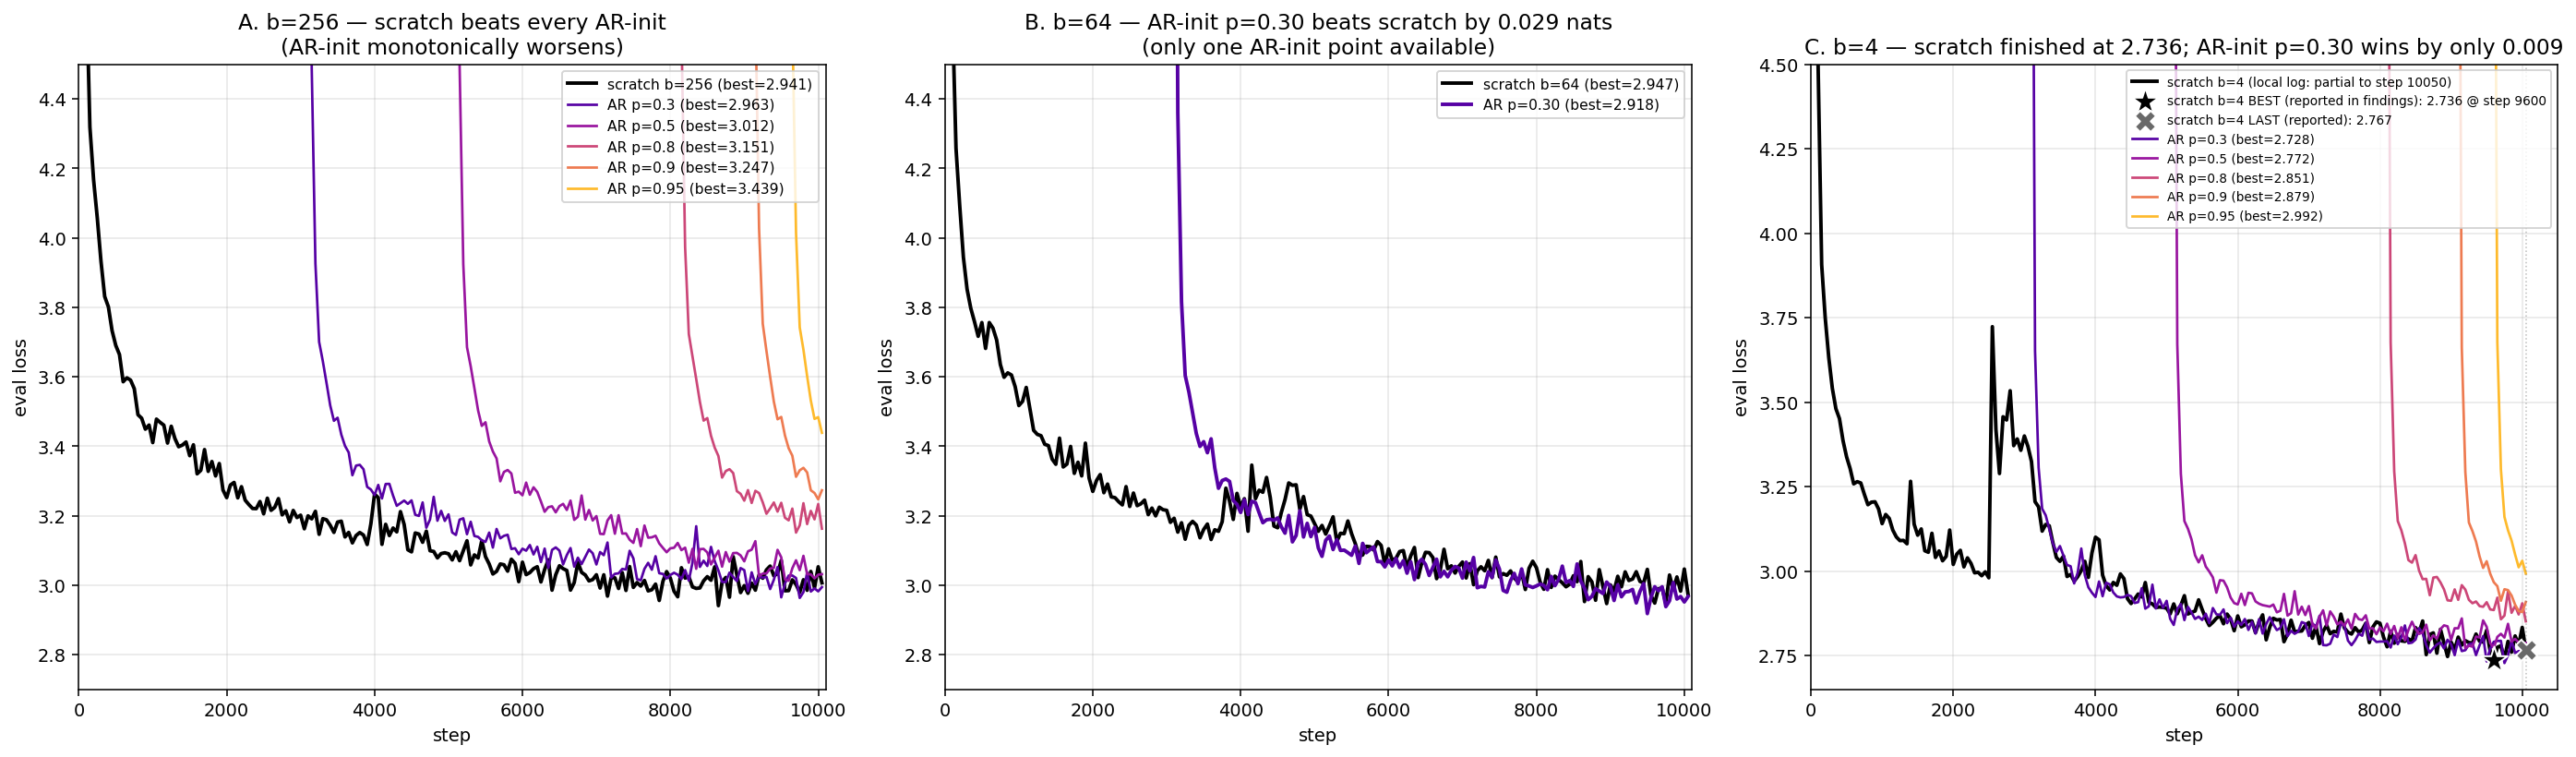
\includegraphics[width=\linewidth]{ar_vs_scratch.png}
    \caption{AR-init vs.\ scratch BD3 at three block lengths. \textbf{Left}: $b{=}256$ -- scratch beats every AR-init run, monotonically in $p_{\mathrm{AR}}$. \textbf{Middle}: $b{=}64$ -- AR-init at $p{=}0.30$ beats scratch by $\sim$0.029 nats. \textbf{Right}: $b{=}4$ -- scratch finishes at 2.736, AR-init $p{=}0.30$ wins by only 0.009 nats. The two regimes (curriculum-helpful at small $b$, curriculum-harmful at large $b$) are visually clear.}
    \label{fig:ar_vs_scratch}
\end{figure}

\subsection{MDLM-init grid}

\begin{table}[h]
\centering
\caption{MDLM$\to$BD3 grid. Best validation loss across the 10.1k-step run. Bold = best per column. Italic = best per row.}
\label{tab:mdlm_init}
\small
\begin{tabular}{lcccc}
\toprule
$p_{\mathrm{MDLM}}$ & $b{=}4$ & $b{=}16$ & $b{=}64$ & $b{=}256$ \\
\midrule
$0.30$ & \textit{\textbf{2.8219}} & \textit{\textbf{2.9497}} & \textit{\textbf{2.9436}} & 2.9528 \\
$0.50$ & \textit{2.8988} & 2.9610 & 2.9679 & 2.9630 \\
$0.80$ & \textit{2.9185} & 2.9645 & 2.9512 & \textit{\textbf{2.9358}} \\
$0.90$ & \textit{2.9487} & 2.9811 & 2.9667 & 2.9505 \\
$0.95$ & \textit{3.0115} & 3.0292 & 2.9938 & \textit{2.9570} \\
\bottomrule
\end{tabular}
\end{table}

The MDLM-init grid mirrors the AR-init pattern: $p_{\mathrm{MDLM}}{=}0.30$ wins at $b \in \{4, 16, 64\}$; $b{=}256$ prefers a much later switch ($p{=}0.80$).

\textbf{BD3LM recipe is suboptimal.} The published BD3LM recipe~\citep{arriola2025block} corresponds to $p_{\mathrm{MDLM}}{=}0.85$ followed by BD3 at $b \le 32$. At $b{=}4$, our $p_{\mathrm{MDLM}}{=}0.30$ run reaches $2.8219$, while $p_{\mathrm{MDLM}}{=}0.80$ gives $2.9185$ and $p_{\mathrm{MDLM}}{=}0.90$ gives $2.9487$. Linearly interpolating to $p{=}0.85$, the BD3LM recipe would land near $2.93$, i.e.\ ${\sim}3.7\%$ worse than our optimum at the same model shape, sequence length, and total budget. Sequence length 512 matches BD3LM's training setting, so this comparison is direct.

\subsection{Cross-track summary}

\begin{table}[h]
\centering
\caption{Best run at each block length, by curriculum family.}
\label{tab:cross_track}
\small
\begin{tabular}{lcccl}
\toprule
$b$ & Scratch BD3 & Best AR-init & Best MDLM-init & Cross-track winner \\
\midrule
$4$   & $2.7364$ & $\mathbf{2.7275}$ ($p{=}0.30$) & $2.8219$ ($p{=}0.30$) & AR-init ($p{=}0.30$) \\
$16$  & ---      & $\mathbf{2.8761}$ ($p{=}0.30$) & $2.9497$ ($p{=}0.30$) & AR-init ($p{=}0.30$) \\
$64$  & $2.9467$ & $\mathbf{2.9179}$ ($p{=}0.30$) & $2.9436$ ($p{=}0.30$) & AR-init ($p{=}0.30$) \\
$256$ & $2.9408$ & $2.9629$ ($p{=}0.30$) & $\mathbf{2.9358}$ ($p{=}0.80$) & MDLM-init ($p{=}0.80$) or scratch \\
\bottomrule
\end{tabular}
\end{table}

The overall best run is \texttt{ar\_p030\_b4\_lr2\_full} at $2.7275$, which beats same-block scratch BD3 by $0.32\%$ and same-block MDLM-init by $3.3\%$. The most striking feature is the column structure: $p_{\mathrm{AR}}{=}0.30$ is winning regardless of the post-switch block length, except at $b{=}256$.

%=============================================================================
\section{Analysis}
\label{sec:analysis}
%=============================================================================

\subsection{The block-length invariance of the optimum}

In both the AR-init and MDLM-init grids, $p{=}0.30$ wins at every block length $b \le 64$. Naively this is surprising: at $b{=}4$ the post-switch task is nearly autoregressive (one masked block of 4, conditioned on clean past blocks), so a strong AR prior should be valuable, suggesting $p_{\mathrm{AR}}$ should be \emph{large}. At $b{=}64$ the post-switch task is much less AR-like, so the AR prior should be \emph{less} useful, suggesting $p_{\mathrm{AR}}$ should be \emph{smaller}. Empirically the optimum is the same.

\subsection{A front-loaded transfer hypothesis}

We propose the following two-ingredient explanation:

\paragraph{(A) AR's marginal value is concave and front-loaded.} Our AR source-chain checkpoints reach validation losses $2.83$ at step $3{,}099$, $2.74$ at $5{,}099$, $2.68$ at $8{,}099$, and $2.66$ at $9{,}099$ on the AR objective itself. The bulk of AR's gain happens within the first ${\sim}30\%$ of the budget; subsequent steps deliver log-shaped diminishing returns on language fundamentals already acquired.

\paragraph{(B) BD3 has slow-converging task-specific structure.} BD3LM's loss curve in scratch and post-switch runs continues to improve through 10k steps; mask handling, mixed clean+noisy contexts, and bidirectional intra-block attention are skills the AR phase never teaches. Late switches starve this adaptation phase.

The optimal switch point is the budget allocation where the marginal value of AR drops below the marginal value of BD3-specific adaptation. Crucially, this crossover is governed by AR-side dynamics: the AR phase is identical regardless of the post-switch block length, so the optimal $p^\star$ is approximately invariant in $b$. This explains the most striking pattern in our data.

\paragraph{The $b{=}256$ exception is also predicted.} At half-sequence block, the BD3 post-switch task is so distributionally far from AR that AR features fail to transfer at all (Figure~\ref{fig:b256}). With near-zero transfer, every step of AR pretraining is opportunity-cost relative to BD3 adaptation, and scratch BD3 wins. MDLM-init partially recovers because MDLM features are themselves diffusion-flavored, so MDLM$\to$BD3 retains some transferability even at large $b$.

\begin{figure}[t]
    \centering
    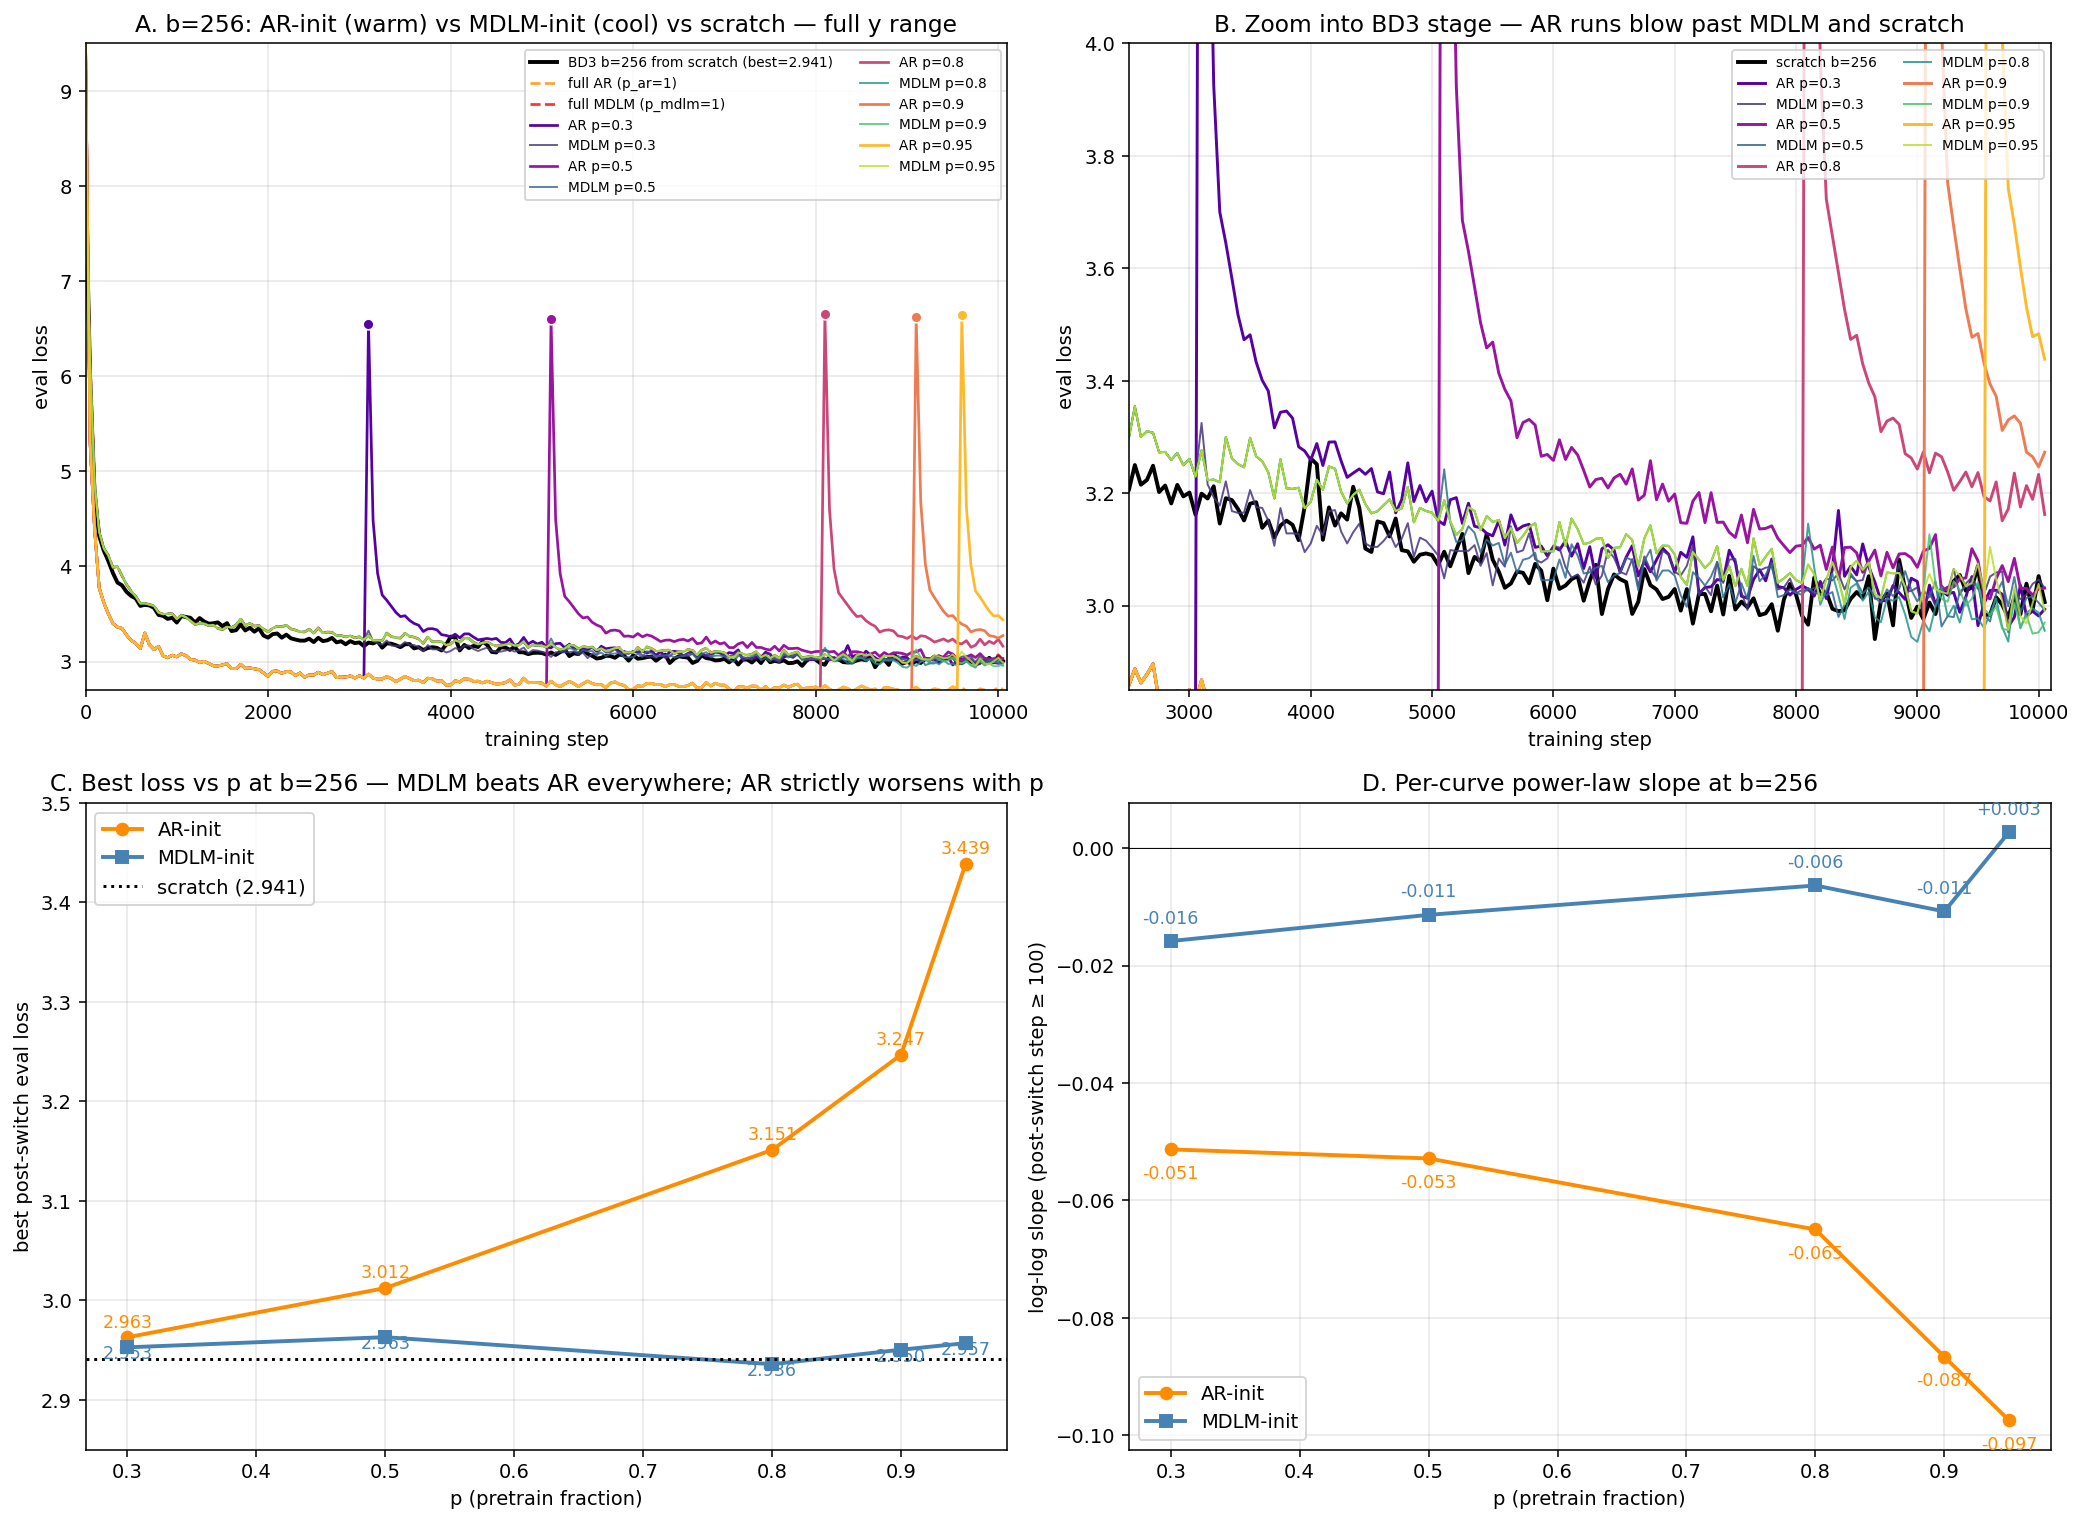
\includegraphics[width=\linewidth]{loss_curves_b256.png}
    \caption{$b{=}256$. \textbf{(A)} Full eval-loss curves: AR-init runs blow past MDLM-init and scratch immediately after the switch; only at very early switches do they recover. \textbf{(C)} Best post-switch eval vs.\ $p$: MDLM-init beats AR-init at every $p$, and AR-init worsens monotonically with $p$. \textbf{(D)} Per-curve power-law slope: AR-init's slope flattens (worse decay) as $p$ grows. The pattern inverts the small-$b$ pattern.}
    \label{fig:b256}
\end{figure}

\subsection{AR-init vs.\ MDLM-init at $b{=}4$}

\begin{figure}[t]
    \centering
    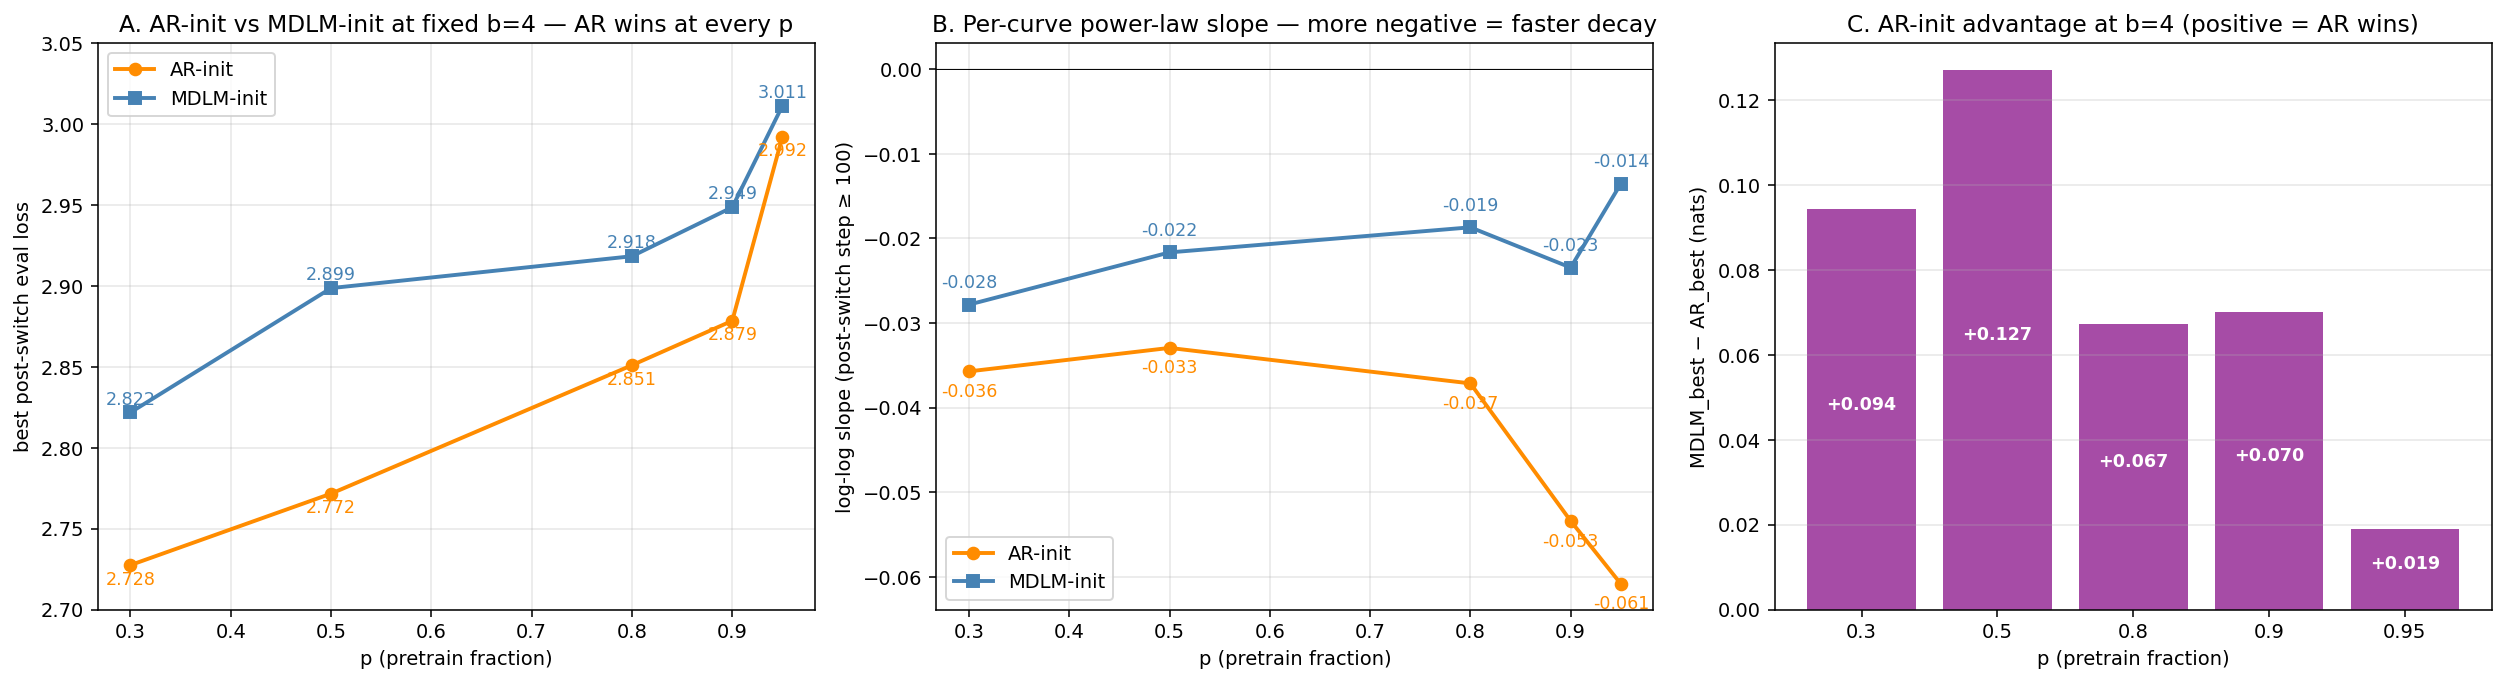
\includegraphics[width=\linewidth]{ar_vs_mdlm_b4.png}
    \caption{AR-init vs.\ MDLM-init at $b{=}4$. \textbf{(A)} Best post-switch loss as a function of $p$: AR-init dominates at every $p$. \textbf{(B)} Per-curve log-log slope (more negative $=$ faster decay): MDLM-init has shallower slopes throughout. \textbf{(C)} AR-init advantage in nats at $b{=}4$: positive at every $p$, peaking at $+0.127$ at $p{=}0.5$.}
    \label{fig:ar_vs_mdlm}
\end{figure}

At $b{=}4$, AR-init beats MDLM-init at every $p \in \{0.30, 0.50, 0.80, 0.90, 0.95\}$ (Fig.~\ref{fig:ar_vs_mdlm}C). This is consistent with the front-loaded-transfer hypothesis: the AR objective produces features that are more directly usable for small-block BD3 (which is itself nearly AR), while MDLM features encode bidirectional context use that is less aligned with $b{=}4$ BD3.

\subsection{MoE health does not confound the loss results}

Late-switch AR-init runs at $b{=}4$ show progressively higher MoE-dropped-token fractions and lower router entropy (drop $0.00004 \to 0.022$, entropy $1.226 \to 1.110$ from $p{=}0.30$ to $p{=}0.95$). Late switches are unhealthy not just on validation loss but also on routing diagnostics, ruling out the alternative hypothesis that the loss differences come from coincidental MoE collapse.

%=============================================================================
\section{Data-Constrained Validation \TODO{run}}
\label{sec:data_constrained}
%=============================================================================

The results above are at compute-bound scale (${\sim}1.7$ epochs over $1.54$B unique tokens). The original motivation for studying dLMs is the data-constrained regime, where AR overfits in multi-epoch training while diffusion continues to improve~\citep{ni2025diffusionlanguagemodelssuper, gao2025whatmakes}. We therefore plan a small data-constrained experiment to verify that the curriculum optimum remains valid where it most matters.

\paragraph{Setup.} We hold the model and optimizer identical to Section~\ref{sec:method}, fix the unique-data pool $U \in \{25\text{M}, 50\text{M}, 100\text{M}\}$ tokens (drawn from ClimbMix held-in shards), and train each method to convergence under heavy regularization. The AR baseline is properly tuned via a Muon weight-decay sweep at each $U$ (we already know from \texttt{dense\_data\_limited.md} and \texttt{moe\_data\_limited.md} that the default config overfits hard at $U{=}25$M; without WD tuning the AR baseline is artificially weak). Methods compared:

\begin{itemize}
\item AR, with per-$U$ best Muon WD.
\item Scratch BD3 ($b{=}4$), with per-$U$ best Muon WD.
\item Curriculum AR$\to$BD3 ($p_{\mathrm{AR}}{=}0.30$, $b{=}4$), with the AR-phase WD chosen from the AR sweep at the same $U$.
\end{itemize}
Each method is run with 2 seeds; we report best validation loss with checkpoint saving enabled (the current MoE data-limited runs have checkpoints disabled, which makes their best-eval claims unrecoverable).

\paragraph{What success looks like.} The curriculum claim survives if at every $U$, $p_{\mathrm{AR}}{=}0.30$ matches or beats both scratch BD3 and tuned AR on best validation loss. The result we are most worried about is that tuned AR closes the gap to scratch BD3 (or beats it) at $U{=}25$M, in which case the data-constrained advantage of dLMs may itself be partly a hyperparameter artifact rather than a fundamental property.

\TODO{Insert results table for AR / Scratch BD3-b4 / Curriculum p=0.30,b=4 at $U \in \{25\text{M}, 50\text{M}, 100\text{M}\}$. Plot best-eval-vs-$U$ for the three methods. See \texttt{moe\_data\_limited.md} \S Next Steps for the launch plan.}

%=============================================================================
\section{Limitations}
\label{sec:limitations}
%=============================================================================

\textbf{One model size.} All curriculum results are at 70M parameters. Whether $p^\star{=}0.30$ holds at 150M+ is open; we plan a single 150M scale-up at compute-optimal as a generalization check.

\textbf{Single total budget.} The grid is at $T{=}10{,}100$ steps. Whether the optimum is invariant to total budget is testable but not yet tested.

\textbf{Validation loss only.} We do not report downstream metrics (HellaSwag, ARC, etc.). At 70M / $\le$2.65B tokens, downstream signal is near-noise on standard benchmarks; the data-constrained scaling planned in \S\ref{sec:data_constrained} is the appropriate follow-up.

\textbf{AR-init grid is partially populated at $b{=}16, 64$.} Only $p_{\mathrm{AR}}{=}0.30$ is run at these block lengths in the AR-init track. The MDLM-init grid (full 5$\times$4) and the AR-init full sweep at $b \in \{4, 256\}$ jointly support the invariance claim, but a complete AR-init grid would tighten the case.

\textbf{Comparison to BD3LM is at our setup, not theirs.} Our $p_{\mathrm{MDLM}}{=}0.85$-recipe estimate is from interpolating our own grid, not from re-running their full recipe with their data and tokenizer.

%=============================================================================
\section{Conclusion}
\label{sec:conclusion}
%=============================================================================

Treating the AR-to-diffusion conversion ratio as a tunable hyperparameter rather than a fixed design choice changes the answer. At 70M MoE / ClimbMix / sequence length 512 / 10.1k steps, the validation-loss-optimal switch point is $p_{\mathrm{AR}}{=}0.30$, invariant in the BD3 post-switch block length except at $b{=}256$. The optimum is much earlier than the $p_{\mathrm{AR}} \approx 0.85\text{--}0.99$ implied by current A2D recipes (BD3LM, Dream-7B, SDAR, LLaDA-2). A simple front-loaded transfer hypothesis explains both the interior optimum and its block-length invariance. Whether this finding translates to larger scale and to the data-constrained regime is the natural next test.

\subsubsection*{Acknowledgments}
Experiments were run on shared 4$\times$H100 nodes rented on Vast.ai.

\bibliography{iclr2026_conference}
\bibliographystyle{iclr2026_conference}

\appendix

%=============================================================================
\section{LR-multiplier probes}
\label{app:lr}
%=============================================================================

We selected $\mathrm{lr\_mult}$ by short probes prior to the main grid.

\begin{table}[h]
\centering
\caption{LR-multiplier probes for MDLM$\to$BD3 switches. Probe length $1500$ steps, $p{=}0.30$, $b{=}64$. \texttt{lr\_mult=0.6667} chosen.}
\small
\begin{tabular}{lcl}
\toprule
$\mathrm{lr\_mult}$ & Best eval & Notes \\
\midrule
0.22   & 3.1716 & Too slow/low, terminated \\
0.6667 & \textbf{3.0973} & Selected \\
2.00   & 3.1318 & Viable but worse \\
6.00   & 3.3373 & Bad, terminated \\
\bottomrule
\end{tabular}
\end{table}

The AR$\to$BD3 switch uses $\mathrm{lr\_mult}{=}2.0$, which matches the scratch BD3LM baseline LR. The asymmetry between the two switch tracks is consistent with MDLM features sitting closer to BD3 in optimization geometry, so a smaller LR is needed to avoid disturbing them.

%=============================================================================
\section{Source-chain training}
\label{app:source}
%=============================================================================

To enable curriculum runs at the same $p$ to share the source-objective phase, we trained one AR source chain and one MDLM source chain to $T{=}10{,}100$ steps and saved checkpoints at the budgeted switch points $\{p{=}0.30, 0.50, 0.80, 0.90, 0.95, 1.00\}$. Source-chain best validation losses on their native objectives are summarized below; switch runs branch from these checkpoints with the appropriate LR multiplier and post-switch objective.

\begin{table}[h]
\centering
\caption{Source-chain checkpoints. ``Best eval'' is on the source objective.}
\small
\begin{tabular}{lcrr}
\toprule
Source run & Final step & Best eval & Best step \\
\midrule
\texttt{source\_ar\_to03100}   & 3099  & 2.8273 & 3050 \\
\texttt{source\_ar\_to05100}   & 5099  & 2.7419 & 5050 \\
\texttt{source\_ar\_to08100}   & 8099  & 2.6792 & 7100 \\
\texttt{source\_ar\_to09100}   & 9099  & 2.6610 & 8950 \\
\texttt{source\_ar\_to10100}   & 10099 & 2.6718 & 9900 \\
\midrule
\texttt{source\_mdlm\_to03100} & 3099  & 3.2299 & 3050 \\
\texttt{source\_mdlm\_to05100} & 5099  & 3.1484 & 4850 \\
\texttt{source\_mdlm\_to08100} & 8099  & 3.0349 & 7500 \\
\texttt{source\_mdlm\_to09100} & 9099  & 2.9861 & 9000 \\
\texttt{source\_mdlm\_to10100} & 10099 & 2.9704 & 9750 \\
\bottomrule
\end{tabular}
\end{table}

The AR source chain is much stronger than the MDLM source chain on their respective native objectives, but this does not translate into post-switch BD3 superiority for late switches: in both grids, $p{=}0.30$ wins.

\end{document}
